\section{Health and Immunity}

\begin{multicols}{2}


\subsection{Coughs and Sneezes \hfill \\ Spread Diseases} % VSO 58, Source 121

\begin{center}
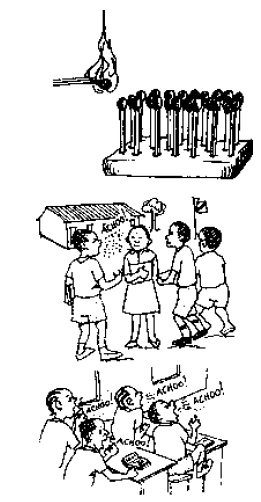
\includegraphics[width=0.4\textwidth]{./img/source/coughs.png}
\end{center}

\begin{description*}
%\item[Subtopic:]{}
%\item[Materials:]{}
%\item[Setup:]{}
\item[Procedure:]{Place the matches in the match box as shown and ignite one.}
%\item[Hazards:]{}
\item[Questions:]{Why is it dangerous to sneeze or cough without covering the mouth or nose?}
%\item[Observations:]{}
\item[Theory:]{Moisture may be seen leaving an uncovered mouth or nose. The water droplets contain
microbes. If one is suffering from an airborne disease such as influenza or tuberculosis
sneezing or coughing could be a source of spreading the harmful microbes. It is necessary to
be aware of this when coughing/sneezing, so that we do not spread the germs to others.
}
\item[Applications:]{Doctors and nurses wear masks to stop germs from their noses and mouths getting on to
people having operations or on to newborn babies.}
%\item[Notes:]{}
\end{description*}

\subsection{Smoking and Health}

\begin{center}
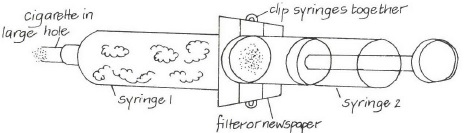
\includegraphics[width=0.45\textwidth]{./img/vso/smoking.jpg}
\end{center}

\begin{description*}
%\item[Subtopic:]{}
\item[Materials:]{2 syringes, filter paper, cigarette}
%\item[Setup:]{}
\item[Procedure:]{Remove the needle end from one syringe (syringe 2). Remove the
plunger from the other syringe (syringe 1) and make a larger hole in
the needle end. Join the syringes as shown. Place a piece of filter paper
or newspaper between the 2 syringes. Place the cigarette in syringe 1
and light it. Draw air through the cigarette several times.}
%\item[Hazards:]{}
\item[Observations:]{You will
see a dark stain spreading across the filter paper. This is tar from the cigarette.}
\item[Questions:]{Ask students what happens to the tar if a person smokes the cigarette and discuss its effect on health.}
%\item[Theory:]{}
%\item[Applications:]{}
%\item[Notes:]{}
\end{description*}

\subsection{Water Baby} % VSO 58

\begin{center}
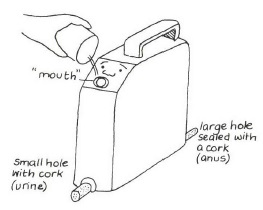
\includegraphics[width=0.4\textwidth]{./img/vso/water-baby.jpg}
\end{center}

\begin{description*}
%\item[Subtopic:]{}
\item[Materials:]{Plastic bottle, 2 corks, water}
%\item[Setup:]{}
\item[Procedure:]{Make a model baby from the bottle. The hole in the top
represents the mouth. Make
a small hole at the bottom to represent water loss through urine and a large hole
to represent the anus. Put corks in both holes. Fill the `baby' with
water. }
%\item[Hazards:]{}
%\item[Questions:]{}
\item[Observations:]{Remove the smaller plug and
water will be lost slowly.
However, diarrhea can cause
severe loss of water, as removing
the larger plug illustrates. }
\item[Theory:]{Water
lost through the holes can only be
replaced through the `mouth'. lf more water is lost than is taken in dehydration occurs and this can
be fatal especially in small babies.}
%\item[Applications:]{}
%\item[Notes:]{}
\end{description*}

\subsection{Oral Rehydration Solution}

\begin{center}
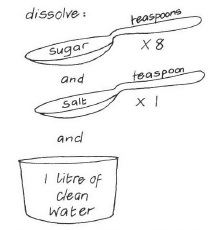
\includegraphics[width=0.4\textwidth]{./img/vso/ors.jpg}
\end{center}

\begin{description*}
%\item[Subtopic:]{}
\item[Materials:]{1 L clean water, 8 teaspoons sugar, 1 teaspoon salt}
%\item[Setup:]{}
\item[Procedure:]{Combine the materials to make an Oral Rehydration Solution (ORS) to help treat diarrhea.}
%\item[Hazards:]{}
%\item[Questions:]{}
%\item[Observations:]{}
\item[Theory:]{Our bodies need water to function normally,
but we also need a particular concentration of essential electrolytes,
e.g. sodium and potassium. These electrolytes are lost in diarrhea and
they must be replaced. Drinking water alone will not save the life of a
person who is dehydrated and has lost too many electrolytes. To
replace some essential electrolytes and water, the baby, or adult,
should drink the Oral Rehydration Solution (ORS)
shown here.}
%\item[Applications:]{}
\item[Notes:]{This is an emergency solution and does not contain
all electrolytes. A severely dehydrated baby may need a
more complex solution if diarrhea persists.}
\end{description*}

\vfill
\columnbreak

\subsection{HIV Acting} % VSO 59

\begin{center}
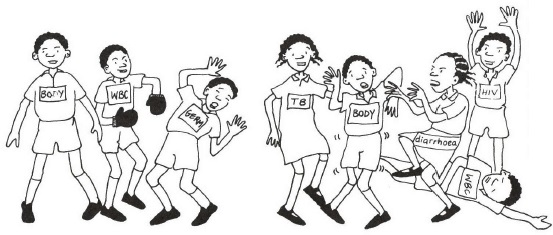
\includegraphics[width=0.4\textwidth]{./img/vso/hiv-acting.jpg}
\end{center}

\begin{description*}
%\item[Subtopic:]{}
\item[Materials:]{Cards, pins/tape}
%\item[Setup:]{}
\item[Procedure:]{Make cards to attach to students. They should contain a mixture of the
following - HIV; diseases, e.g. TB, diarrhea; white blood cell. One of
the pupils should represent the human body. Several `white blood cells'
should be protecting one body' to begin with. Ask students to act out
the spread of HlV.}
%\item[Hazards:]{}
%\item[Questions:]{}
%\item[Observations:]{}
\item[Theory:]{White blood cells protect the
body from diseases. HIV knocks
out the white blood cells and so
they can no longer protect the
body. This leaves the body open
to attack by germs of all kinds.
Eventually the body is overcome
by diseases which are normally
not fatal.}
%\item[Applications:]{}
%\item[Notes:]{}
\end{description*}

\subsection{Passing On HIV}

\begin{center}
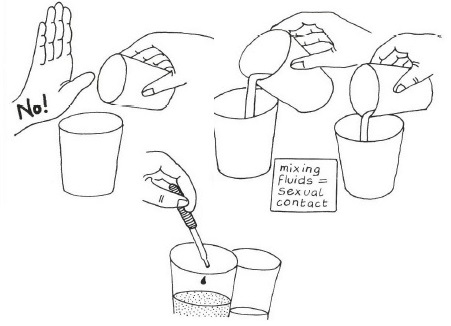
\includegraphics[width=0.4\textwidth]{./img/vso/hiv-passing.jpg}
\end{center}

\begin{description*}
%\item[Subtopic:]{}
\item[Materials:]{Cards, starch solution, iodine solution}
\item[Setup:]{On the cards write down some sexual case histories. Give each student
a card at random. The owner of the card is to follow the behaviour
indicated on the card, e.g. faithful to one partner, many partners, no
partners. }
\item[Procedure:]{Give a few of the students a cup of starch solution and give
all the others a cup of water. Ask students to follow the case history of
the cards and to mix the contents of their cups when they have a
partner - mixing represents sexual contact. At some point `HlV test' the
contents of the cups using a few drops of iodine solution. lf the
solution goes dark then it means there is starch (representing HIV) in
the cup.}
%\item[Hazards:]{}
%\item[Questions:]{}
\item[Observations:]{Discuss how fast the virus
spreads. Also discuss how its
spread could be prevented or
slowed down.}
%\item[Theory:]{}
%\item[Applications:]{}
%\item[Notes:]{}
\end{description*}

%==================================================================================================%


\end{multicols}

\pagebreak